Here we derive an expression for the Bernoulli parameter, \be
\mathcal{B} \equiv \ke +\gammaf \frac{p}{\rho}+\Phi, \ee
as a function of radius $x \equiv r/\rs$.  Straightforward manipulation of the hydrodynamic equations (eqs.~[\ref{eq:drhodt}]-[\ref{eq:dsdt}]) results in the following relationship: 
\begin{align}
\frac{1}{r^2} \frac{d}{dr} \left(r^2 \rho v \mathcal{B} \right) = q \kew + q \Phi,
\label{eq:enCons}
\end{align}
which upon integration from the stagnation radius $r = \rs$ outwards,
\begin{align}
  r^2 \rho v(\mathcal{B} - \mathcal{B}|_{\rs})= \int_{\rs}^{r}
    r^2 \left(\frac{3}{1+\delta}\frac{G
  \Mbh}{r}+\sigma_0^2+v_w^2 + q \Phi\right) dr,
    \label{eq:enConsInt}
\end{align}
where the right hand side makes use of the definition of $\vw^{2}$ (eq.~[\ref{eq:sigmarel}]).

The mass flux follows from mass continuity (eq.~[\ref{eq:drhodt}]) and the condition that $v|_{\rs} = 0$:
\begin{equation}
 \drhodt+\frac{1}{r^2}\frac{\partial}{\partial r}\left(\rho r^2 v\right)=q \Rightarrow r^2 \rho v = q_o \rs^3 \left[\frac{x^{3-\delta}-1}{3-\delta}\right],
 \label{eq:massFlux}
 \end{equation}
where the source term obeys $q = q_o x^{-\delta} \propto \rho_{\star} \propto r^{-1-\Gamma}$ and $\delta \equiv -1-\Gamma$.  The gravitational potential $\Phi$ is given by
\begin{align}
\Phi \simeq -\frac{G \Menc}{r} -4 \pi G \int_{r}^{\rb} \rhostar(r') r' dr',
\label{eq:Phi}
\end{align}
where by truncating the integral at $r = \rb$ we neglect contributions to the potential from stars outside of the break radius, as is generally a good assumption.

Tedious but straightforward manipulation of equations~\eqref{eq:enConsInt}, \eqref{eq:massFlux}, \eqref{eq:Phi}, results in the following:
\begin{align}
  &\mathcal{B} = -U_o\left[\frac{\rs/\rb}{2-\delta}-\frac{x^{5-2\delta}-1}{x^{3-\delta}-1}\frac{3-\delta}{(5-2\delta)(2-\delta)}\right]\nonumber\\
  &+\frac{v_w^2}{2}+\frac{\sigma_0^2}{2}- \frac{G \Mbh}{r_s}
  \frac{1-2\delta}{2(\delta+1)}
  \frac{3-\delta}{2-\delta}\frac{x^{2-\delta}-1}{x^{3-\delta}-1}
  \nonumber\\
  &-\frac{G M_\star}{r_s}
  \frac{x^{5-2\delta}-1}{x^{3-\delta}-1}\frac{3-\delta}{5-2\delta},
\end{align}
where $U_o=4 \pi G \rhostar|_{\rs} \rs^2$.  This can be rewritten as
\begin{multline}
  \mathcal{B} =\frac{G \Mbh}{\rs} \biggl[ \frac{3}{2} \zeta^2
  w^{\frac{1}{3 -\delta}}
  -\frac{(1-2\delta)(3-\delta)}{2(\delta+1)(2-\delta)}  \frac{x^{2  -\delta}-1}{x^{3-\delta}-1}\\
  -\frac{\rb}{\rsoi} w^{\frac{\delta-1}{3-\delta}} \frac{3 -\delta}{2
    -\delta} -w
  \frac{(2-\delta)(3-\delta)-(3-\delta)^{2}}{(5-2\delta)(2-\delta)}
  \frac{x^{5-2\delta}-1}{x^{3-\delta}-1} \biggr],
\label{eq:enthAnal}
\end{multline}
where $\zeta \equiv \sqrt{1 + (v_w/\sigma_0)^2}$ and $w\equiv
(\rs/\rsoi)^{3\delta}$.

Analysis of equation (\ref{eq:enthAnal}) results in the following interpretation of the behavior of the Bernoulli integral as a function of the heating rate.  When the rate of external heating is high ($\zeta \gg 1$), then $\mathcal{B} > 0$ at all radii, requiring an outflow with positive kinetic energy at infinity.  However, as $\zeta$ is decreased, there exists a critical value of $\zeta = \zeta_{c}$ below which $\mathcal{B}$ becomes negative; this occurs first near the stagnation radius and then the region where $\mathcal{B} < 0$ grows to larger radii as $\zeta$ is reduced further.  If $\zeta$ is just less than $\zeta_c$, then we can have still $\mathcal{B} > 0$ at the break radius, allowing an outflow with positive asymptotic kinetic energy, but only if $\rs$ exceeds a minimum value, $r_{\rm s,min}$.  

The critical heating value $\zeta_c$ is an increasing function of $r_{b}/r_{\rm soi}$ and is larger for core galaxies than cusp galaxies, since a greater heating rate is required to unbind gas from a deeper stellar potential (Fig.~\ref{fig:zetaCrit}).  Specifically, we find $\zeta_c\sim (\rb/\rsoi)^{0.5(1-\Gamma)}$ for $\rb\gsim\rsoi$ (see the top panel of Fig.~\ref{fig:zetaCrit} for the case of core galaxies). Likewise the minimum $r_{\rm s,min}/r_{b}$ is an increasing function of $\zeta/\zeta_{c}$, approaching unity for $\zeta < 0.86\zeta_c$, as shown in the bottom panel of Fig.~\ref{fig:zetaCrit}.  As $\zeta \rightarrow 0.86\zeta_c$ our numerical simulations show that that the stagnation radius diverges from its value predicted by equations (\ref{eq:stag_analytic}) and (\ref{eq:densSlope}) and moves out to the break radius.  


\begin{figure}
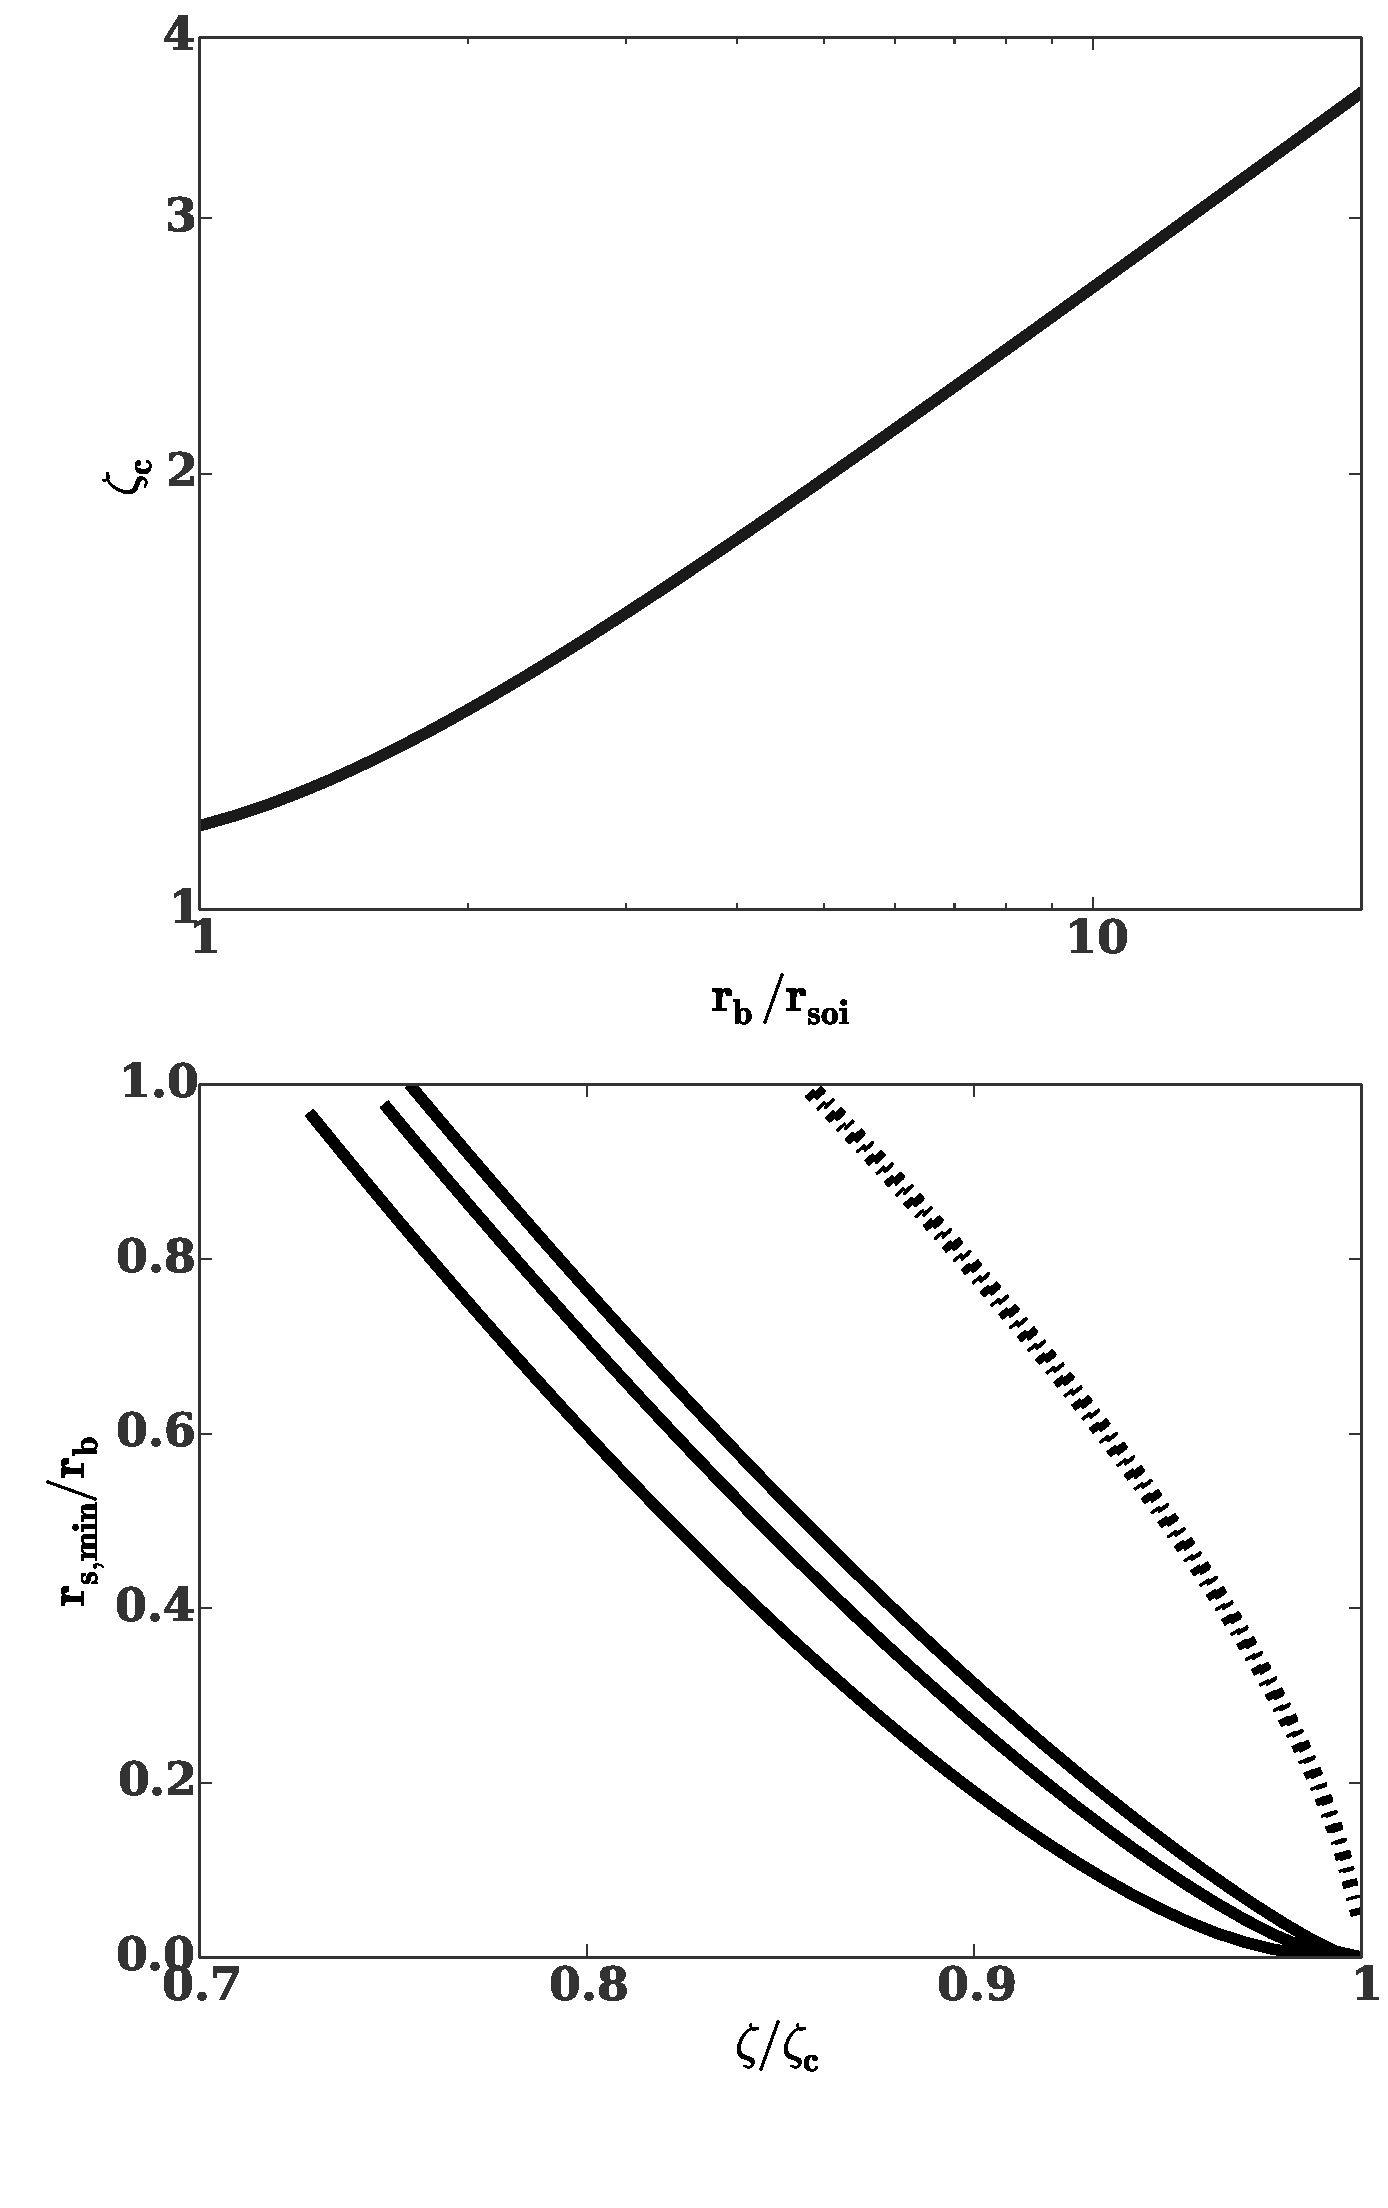
\includegraphics[width=\columnwidth]{zetaCrit.pdf}
\caption{\label{fig:zetaCrit} {\emph Top panel:} Critical
  $\zeta_c=\sqrt{v_w^2+\sigma_0^2}/\sigma_0$ for core ($\Gamma=0.1$)
  galaxies. If $\zeta<\zeta_c$ outflows are only possible if the ratio
  of the stagnation radius to the influence radius exceeds a minimum
  value. Plotted as a function of the ratio of the break radius to the
  influence radius ($\rb/\rsoi$) {\emph Bottom Panel:} Mininmum value
  for ratio of the stagnation radius to the break radius, $\rs/\rb$
  for core galaxies ($\Gamma=0.1$) derived by requiring the Bernoulli
  parameter of the gas to remain positive out to the break radius
  $\rb$. This is calculated numerically from
  equation~\eqref{eq:enthAnal}.}
\end{figure}


%%% Local Variables: 
%%% mode: latex
%%% TeX-master: "ms"
%%% End: 
